%	Plattformabhängikeit   & 0   & 1 & 2       & 3 & 4  & 10\%         \\
%Installation           & 0   & 1 & 2       & 3 & 4  & 5\%          \\
%Speicherzugriff        & 0   & 1 & 2       & 3 & 4  & 5\%          \\
%Speicherbedarf         & 0   & 1 & 2       & 3 & 4  & 5\%          \\
%Aktualisierbarkeit     & 0   & 1 & 2       & 3 & 4  & 5\%          \\
%Konsistenz des Designs & 0   & 1 & 2       & 3 & 4  & 5\%         \\
%Bibliotheken           & 0   & 1 & 2       & 3 & 4  & 10\%         \\
%Umsetzung              & 0   & 1 & 2       & 3 & 4  & 20\%         \\
%Testbarkeit            & 0   & 1 & 2       & 3 & 4  & 10\%         \\
%Vorausgesetzte Entwicklungserfahrung    & 0   & 1 & 2       & 3 & 4  & 10\%         \\
%Verständlichkeit       & 0   & 1 & 2       & 3 & 4  & 10\%         \\
%
\begin{figure}[h]

	\begin{tikzpicture}
	
		% Diagram setup
		\tkzKiviatDiagram[scale=1.0,label distance=.5cm,
		radial  = 4,
		gap     = 1,  
		lattice = 4]{
			Installation,
			Speicherzugriff,
			Speicherbedarf,
			Aktualisierbarkeit,
			Konsistenz des Designs,
			Bibliotheken,
			Umsetzung,
			Testbarkeit,
			Vorausgesetzte Entwicklungserfahrung,
			Nutzerfreundlichkeit
		}
		
		% native App
		\tkzKiviatLine[thick,color=blue,mark=ball,
		fill=blue!20,opacity=.5](4,4,2,3,3,1,2,3,3,4)
		
		% PWA
		\tkzKiviatLine[thick,color=green,mark=ball,
		fill=green!20,opacity=.5](2,3,4,4,1,4,4,4,1,2)
		
		\tkzKiviatGrad[prefix=,unity=1,suffix=](0)  
	

	
	\end{tikzpicture}
	
	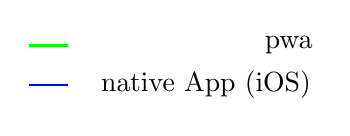
\begin{tikzpicture}
	%\draw[draw=black!20] (-0.1,-0.2) rectangle ++(15,0.5);
	
	\draw [thick, green] (0,0.5) -- (0.5,0.5); 
	\node at (3.3,0.5) {\acf{pwa}};
	
	\draw [thick, blue] (0,0) -- (0.5,0); 
	\node at (2.25,0) {native App (iOS)};
	

		\end{tikzpicture}
	
	\caption{Spinnennetzdiagram}
\end{figure}